\chapter{Algorytm - TODO}
\label{cha:Algorytm}

Niniejszy rozdział skupiać się będzie na algorytmie służącym do rozwiązania problemu, jakim jest wyznaczenie optymalnej prędkości na drodze. Zostaną w nim opisane poszczególne składowe wchodzące w jego skład, takie jak:
\begin{itemize}
\item przyporządkowanie obiektów reprezentowanych przez punkty, do poszczególnych dróg
\item przyporządkowanie obiektów reprezentowanych przez dwuwymiarowe figury geometryczne, do poszczególnych dróg
\item wyznaczanie dopuszczalnej prędkości
\item odpowienie umiejscowienie znaków
\end{itemize}

Dodatkowo, w celu lepszej wizualizacji problemu, zostaną umieszczone zdjęcia, przedstawiające działanie poszczególnych części algorytmu.

\newpage
\section{Przyporządkowanie obiektów reprezentowanych przez punkty, do poszczególnych dróg}
\label{sec:ObiektyPunktDrogi}

Jednym z kluczowych elementów działania algorytmu jest odpowiednie przyporządkowanie obiektów drogowych do poszczególnych dróg. W OpenStreetMap reprezentowane są zarówno przez punkty, jak również przez dwuwymiarowe obiekty geometryczne. 


Obiekty z OpenStreetMap reprezentowane przez punkty:
\begin{itemize}
\item przejścia dla pieszych
\item przejazdy kolejowe
\item sygnalizacja świetlna
\end{itemize}


W niniejszej sekcji skupię się na rozwiązaniu problemu jakim jest przyporządkowanie obiektów przedstawianych jako punkty, do poszczególnych dróg. Do tego celu wykorzystam wzór \ref{eq:distancePointLineal}, wyznaczający odległość punktu od prostej.

\begin{figure}[h]
\label{odlegloscPktProsta}
\centering
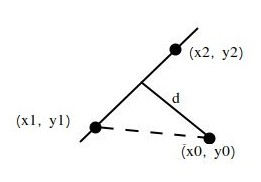
\includegraphics[width=0.5\textwidth]{dlugoscPktOdProstej}
\source{Na podstawie mathworld.wolfram.com}
\end{figure}

Wzór wyznaczający odległość punktu od prostej:

\begin{equation} \label{eq:distancePointLineal}
d = \frac{| (x_2 - x_1)(y_1 - y_0) - (x_1 - x_0)(y_2 - y_1) |}{\sqrt{(x_2 - x_1)^2 + (y_2 - y_1)^2}}
\end{equation}\newline

\begin{itemize}
\item Zmienne: x1, y1, x2, y2 oznaczają współrzędne geograficzne odpowiednio początku i końca drogi. 
\item Zmienne x0, y0 oznaczają współrzędne punktu reprezentujące obiekt drogowy.
\item Zmienna d oznacza najkrótszą odleglość punktu od drogi.  
\end{itemize}


\newpage
\section{Wyznaczanie współrzędnych punktu znajdującego się na drodze, odległego o n metrów od innego punktu}
\label{sec:pointCoordinatesFromAnotherPoint}

Istotnym aspektem działania algorytmu jest rozwiązanie problemu wyznaczenie współrzędnych punktu, znajdującego się na drodze, odległego o n metrów od innego punktu.  Jest to niezbędne w sytuacji, gdy np. program musi ustawić na drodze znak ograniczenia prędkości w odległosci n metrów od przejścia dla pieszych.

Do rozwiązania tego zadania, posłużyłem się własnościami trygonometrycznymi.


\begin{figure}[h]
\label{odlegloscPktProsta}
\centering
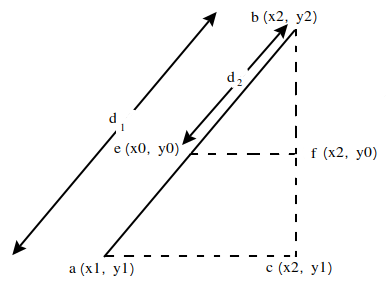
\includegraphics[width=0.5\textwidth]{distance}
\end{figure}

Wiadomym jest, że odległość między dwoma punktami a i b wynosi:
\begin{equation} \label{eq:coordinatesFromPoint}
d_1 = \sqrt{(x1 - x2)^2 + (y1 - y2)^2}
\end{equation}\newline

oraz sinus kąta abc:
\begin{equation} \label{eq:sinABC}
sin_{abc} = \frac{x2 - x1}{d_1}
\end{equation}\newline

jak również sinus kąta ebf:
\begin{equation} \label{eq:sinEBF}
sin_{ebf} = \frac{x2 - x0}{d_2}
\end{equation}\newline

oraz to, że sinusy tego samego kąta są równe:
\begin{equation} \label{eq:sinEBF}
sin_{abc} = sin_{ebf} => \frac{x2 - x1}{d_1} = \frac{x2 - x0}{d_2}
\end{equation}\newline

przez proste przekształcenie, otrzymujemy wzór na współrzędną x0

\begin{equation} \label{eq:x0Coordinates}
x0 = x2 - \frac{d_2*(x2 - x1)}{d_1}
\end{equation}\newline

Wyznaczenie wzoru na współrzędną y0 jest podobne do wyznaczania współrzędnej x0, z tą różnicą, że zamiast sinusa, liczymy cosinusa kąta abc:

\begin{equation} \label{eq:cosABC}
cos_{abc} = \frac{y2 - y1}{d_1}
\end{equation}\newline

oraz cosinusa kąta ebf:
\begin{equation} \label{eq:cosEBF}
cos_{ebf} = \frac{y2 - y0}{d_2}
\end{equation}\newline

a skoro cosinus tego samego kąta są równe:
\begin{equation} \label{eq:cosEBF}
cos_{abc} = cos_{ebf} => \frac{y2 - y1}{d_1} = \frac{y2 - y0}{d_2}
\end{equation}\newline

otrzymujemy równanie współrzędnej y0:
\begin{equation} \label{eq:cosEBF}
y0 = y2 - \frac{d_2*(y2 - y1)}{d_1}
\end{equation}\newline

Przez powyższe obliczenia, wyznaczone zostały wspórzędne poszukiwanego punktu:

\begin{equation} \label{eq:calculatedCoordinates}
(x2 - \frac{d_2*(x2 - x1)}{d_1}, y2 - \frac{d_2*(y2 - y1)}{d_1})
\end{equation}\newline

\newpage
\section{Przyporządkowanie obiektów reprezentowanych przez wielokąty, do poszczególnych dróg}
\label{sec:polygonLineDistance}

\newpage
\section{Przejścia dla pieszych}
\label{sec:pedestrialCrossing}
\subsection{Przyporządkowywanie przejść dla pieszych do poszczególnych dróg}

Bardzo ważnym czynnikiem doboru prędkości jest obecność przejść dla pieszych. Te z sygnalizacją świetlną nie stanowią problemu, ponieważ ruch pieszych poruszających się na nich jest ograniczony tylko do sytuacji, gdy sygnalizacja świeci się na zielono. W przypadku przejść bez sygnalizacji, sprawa się komplikuje, ponieważ kierowca jest zobowiązany do zachowania szczególnej ostrożności i zmiejszenia prędkości od 30 km/h. 

Do przyporządkowania przejść dla pieszych, do poszczególnych dróg, posłużyłem się wzorem \ref{eq:distancePointLineal} na odległość punktu od prostej, przedstawionym w sekcji \ref{sec:ObiektyPunktDrogi}.


Rezultatem wdrożenia powyższego wzoru do programu, są:
\begin{itemize}
\item na niebiesko zaznaczone drogi, na których znajdują się przejścia dla pieszych
\item znakiem ''D-6'' zostały oznaczone przejścia dla pieszych
\end{itemize} 
Wynik został przedstawiony na Rys. \ref{sec:PrzejscieDrogi}:

\begin{figure}[h]
\caption{Drogi na których znajdują się przejścia dla pieszych.}
\label{sec:PrzejscieDrogi}
\centering
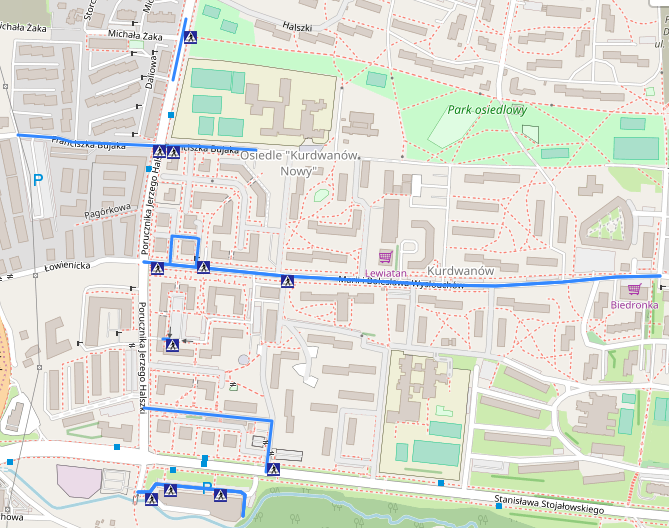
\includegraphics[width=0.9\textwidth]{PrzejscieDrogi}
\end{figure}

Dzięki tak zobrazowanej sytuacji, można ocenić skuteczność algorytmu przyporządkowującego przejścia dla pieszych do określonych dróg.

\subsection{Wyznaczanie prędkości i umieszczanie jej w odpowiednim miejscu na mapie}

Bezpieczna prędkość w pobliżu nieoznakowanych przejść dla pieszych wynosi ok. 30 km/h. Zapewnia ona zarówno wystarczajacy czas reakcji, odpowiednio krótką drogę hamowania oraz zmiejsza ryzyko wystąpień potrąceń pieszych. 

Algorytm umieszcza znaki ograniczenia prędkości:
\begin{itemize}
\item w odległości 50 m od przejścia, gdy maksymalna prędkość na drodze wynosi 60 km/h
\item w odległości 150 m od przejścia, gdy maksymalna prędkość przekracza 60 km/h
\item w przypadku, gdy przejście dla pieszych znajduje się w odległości mniejszej niż 50m lub 150m (w zależności od maksymalnej prędkości), znak zostanie umieszczony na początku drogi
\item w przypadku drogi jednokierunkowej, tylko przed przejściem
\item w przypadku drogi dwukierunkowej, zarówno przed, jak i za przejściem
\item bezpośrednio za przejściem zostanie ustawiony znak przywracającą poprzednie ograniczenie prędkości, za wyjątkiem sytuacji, gdy droga za przejściem dla pieszych jest krótsza niż 100m. W takim wypadku, nie ma sensu zmieniać prędkości. 
\end{itemize}

\begin{figure}[h]
\caption{Ograniczenia prędkości przy przejściach dla pieszych.}
\label{sec:przejsciePredkosci}
\centering
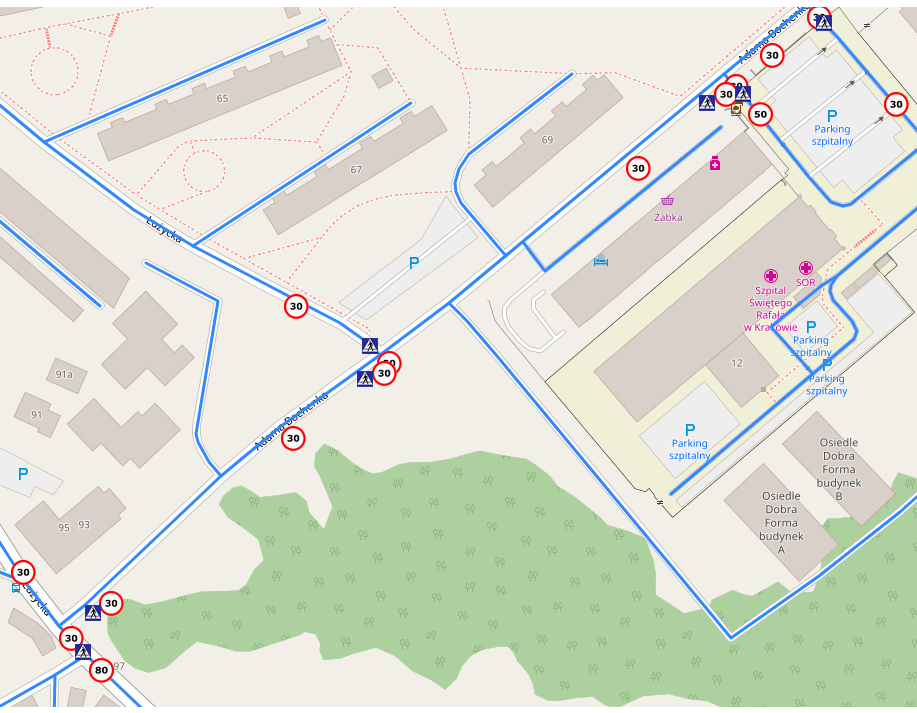
\includegraphics[width=0.9\textwidth]{pedestrian_speed}
\end{figure}

\newpage
\section{Typ nawierzchni}
\label{sec:surfaceType}

W celu zadbania o bezpieczeństwo osób, ale również o dobrą kondycję techniczną pojazdów poruszających się po drogach, niezbędne jest uwzględnienie typu nawierzchni. Nie można dopuścić do sytuacji, gdy na nawierzchni składającej się głównie że żwiru, znajdowało się znak ograniczenia prędkości o wysokiej wartości. Wtedy ulec awarii może zarówno zawieszenie, jak również pojazdy jadące przed nimi pojazdami. Aby zapoabiec tego typu problemom, podzieliłem typ nawierzchni na kilka rodzajów:

\begin{itemize}
\item kostka brukowa
\item żwir
\item drobny żwir
\item nieutwardzana
\item błotnista
\item płyty  betowowe
\item droga gruntowa
\item piasek
\item asfalt
\end{itemize}

Najbardziej problematyczna dla kierowów droga to taka, która pokryta jest żwirem, drobnym żwirem, składająca się z piasku lub jest błotnista. W takich przypadkach ograniczyłem prędkość do 10 km/h. Niewiele lepsza nawierzchnia to taka, która wyłożona jest zarówno kostką brukową oraz płytami betonowymi. Dla nich, odpowiednia prędkość wynosi 20 km/h. W przypadku drogi nieutwardzanej oraz gruntowej, ograniczenie prędkości wynosi 30 km/h. Dla asfaltu, ze względu na jego strukturę, ograniczenie prędkości praktycznie nie występuje. 

Na Rys. \ref{sec:surfaceTypePhoto} zostały umieszczone ograniczenia prędkości dla dróg, których nawierzchnia pokryta jest materiałem innym niż asfalt. Dla celów demonstracyjnych, został on specjalnie pominięty, ponieważ więszkość dróg jest nim pokryta, przez co Rys. \ref{sec:surfaceTypePhoto} stałby się mało czytelny. Oczywiście ogólny algorytm uwzględnia asfalt.

\newpage
\begin{figure}[h]
\caption{Ograniczenia prędkości ze względu na rodzaj nawierzchni.}
\label{sec:surfaceTypePhoto}
\centering
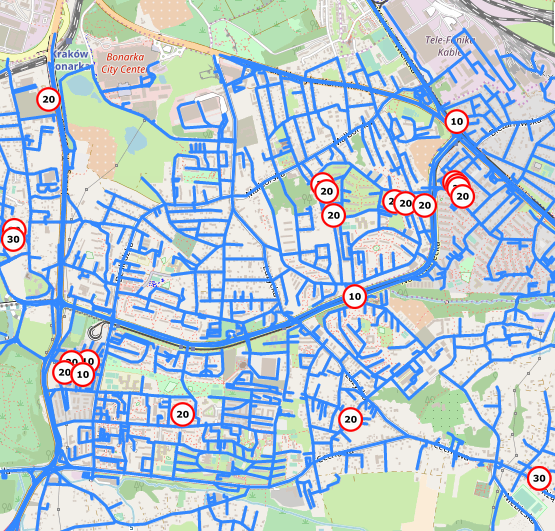
\includegraphics[width=0.9\textwidth]{surfaceType}
\end{figure}

\newpage
\section{Przejazdy kolejowe}
\subsection{Przyporządkowywanie przejazdów kolejowych do poszczególnych dróg}

Istotnych parametrem algorytmu wyznaczającego dopuszczalne prędkości jest obecność przejazdów kolejowych. Jak wiadomo, pociąg nie zatrzyma się w miejscu. Jego droga chamowania w głównej mierze zależy od masy oraz prędkości z jaką się porusza. Dla przykładu, pociąg towarowy o masie ok. 1800 ton, jadący z prędkością ok. 50 km/h, zatrzyma sie po około 500m. Dlatego ważne jest określenie prędkości, z jaką samochód moze się przemieszczać przed takim przejazdem.

Do przyporządkowania przejazdów kolejowych do poszczególnych dróg, wykorzystałem wzór \ref{eq:distancePointLineal} znajdujący się w rozdziale \ref{sec:pedestrialCrossing}


\begin{figure}[h]
\caption{Drogi na których znajdują się przejazdy kolejowe.}
\label{sec:PrzejazdyKolejowe}
\centering
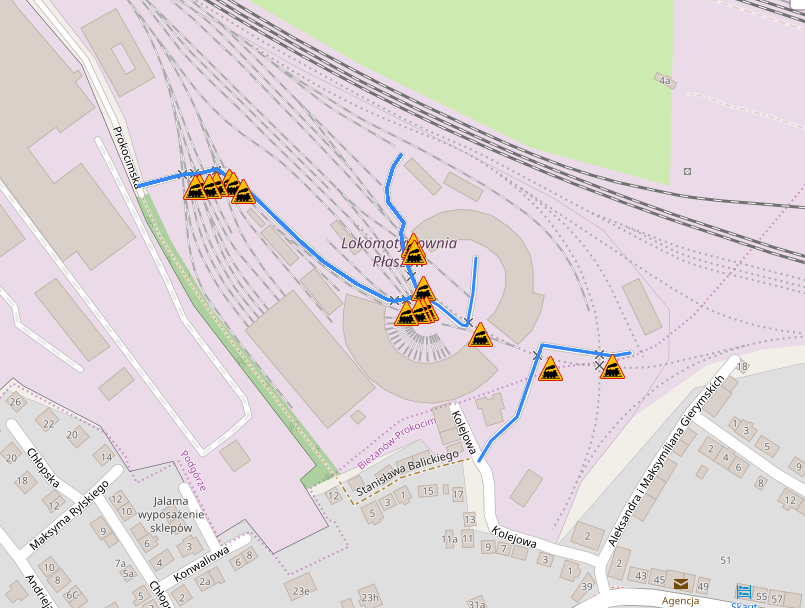
\includegraphics[width=1.0\textwidth]{railCrossing}
\end{figure}

Rys. \ref{sec:PrzejazdyKolejowe} obrazuje wynik przypisania przejazdów kolejowych do poszczególnych dróg:
\begin{itemize}
\item kolorem niebieskim drogi, na ktorych znajdują przejazdy kolejowe
\item znakiem ''A-10'' zostały oznaczone przejazdy kolejowe, pobrane z OpenStreetMap
\end{itemize}

\newpage
\subsection{Wyznaczanie prędkości i umieszczanie jej w odpowiednim miejscu na mapie}

\newpage
\section{Sygnalizacja świetlna}
\subsection{Przyporządkowywanie sygnalizacji świetlnej do poszczególnych dróg}

Aby kierowca bez problemu mógł zdążyć zareagować na zmieniające się swiatło sygnalizacji świetlnej, niezbędne jest zredukowanie prędkości do odpowiedniej wartości. Ze względu na fakt iż sygnalizacja widoczna jest z relatywnie dużej odległości, prędkość przed nią zostanie ograniczona do ok. 50 km/h.


\begin{figure}[h]
\caption{Drogi na których znajduje się sygnalizacja świetlna.}
\label{sec:PrzejazdyKolejowe}
\centering
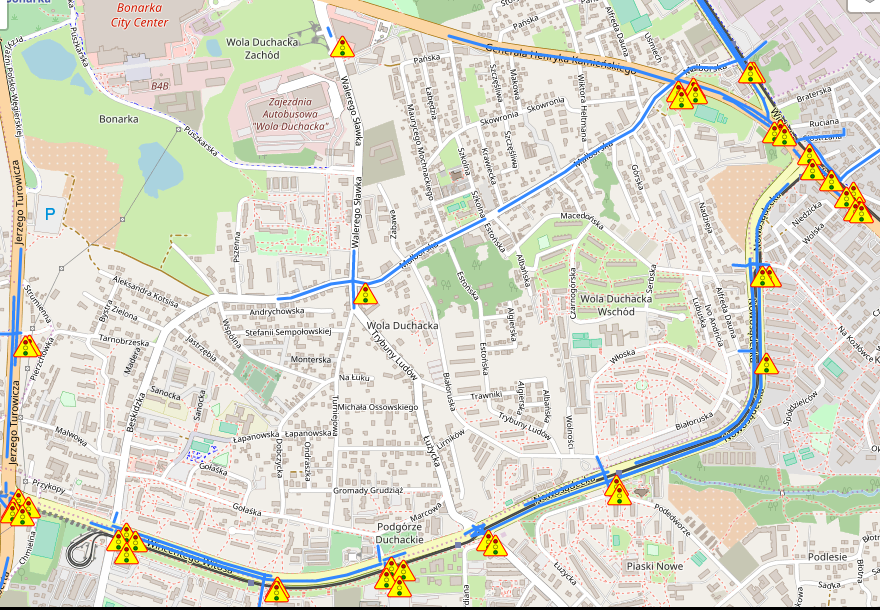
\includegraphics[width=1.1\textwidth]{traffic_sight}
\end{figure}

Rys. \ref{sec:PrzejazdyKolejowe} ukazuje sposób działania algorytmu przypisującego do drogi sygnalizację świetlną. Zaznaczono na nim:
\begin{itemize}
\item kolorem niebieskim drogi, na ktorych znajduje się sygnalizacja świetlna
\item znakiem ''A-29'' zostały oznaczone sygnalizacje świetlne, pobrane z OpenStreetMap
\end{itemize}

\newpage
\subsection{Wyznaczanie prędkości i umieszczanie jej w odpowiednim miejscu na mapie}

\newpage
\section{Przystanki autobusowe i tramwajowe}
\label{sec:zakręty}

\newpage
\section{Szkoły i miesca zabaw}
\label{sec:zakręty}

\newpage
\section{Sklepy i miejsca kultów religijnych}
\label{sec:zakręty}

\newpage
\section{Liczba pasów ruchu}
\label{sec:zakręty}

\newpage
\section{Rodzaj drogi}
\label{sec:zakręty}

\newpage
\section{Płynna zmiana prędkości pojazdów}
\label{sec:zakręty}

\newpage
\section{Historia wypadków}
\label{sec:zakręty}

\newpage
\section{Zakręty}
\label{sec:zakręty}

\section{Umiejscowienie znaków na drodze}
\label{sec:speedLimitLocalization}
Znaki drogowe ograniczenia prędkości są ustawione według następujących kryteriów:
\begin{itemize}
\item na początku każdej drogi
\item przed nieoznakowanymi przejściami dla pieszych
\item przed wjazdem do obszaru, w pobliżu którego znajdują się szkoły, place zabaw, duże sklepy handlowe i miejsca kultów religijnych
\item przed zakrętami
\item między znakami ograniczenia prędkości, dla których występują duże różnice prędkości
\end{itemize}

